%%%%%%%% AURORA Paper - ICML 2026 Format %%%%%%%%%%%%%%%%%

\documentclass{article}

\usepackage{tabularx}

% Recommended packages
\usepackage{microtype}
\usepackage{graphicx}
\usepackage{subcaption}
\usepackage{booktabs}
\usepackage{hyperref}

% For algorithms
\newcommand{\theHalgorithm}{\arabic{algorithm}}

% Use ICML 2026 style (blind submission)
\usepackage{icml2026}

% Math packages
\usepackage{amsmath}
\usepackage{amssymb}
\usepackage{mathtools}
\usepackage{amsthm}

% For plots
\usepackage{pgfplots}
\pgfplotsset{compat=1.18}
\usepgfplotslibrary{groupplots}
\usetikzlibrary{positioning, arrows.meta, shapes, calc, decorations.pathreplacing}

% Cleveref for cross-references
\usepackage[capitalize,noabbrev]{cleveref}

% Theorems
\theoremstyle{plain}
\newtheorem{theorem}{Theorem}[section]
\newtheorem{proposition}[theorem]{Proposition}
\newtheorem{lemma}[theorem]{Lemma}
\newtheorem{corollary}[theorem]{Corollary}
\theoremstyle{definition}
\newtheorem{definition}[theorem]{Definition}
\newtheorem{assumption}[theorem]{Assumption}
\theoremstyle{remark}
\newtheorem{remark}[theorem]{Remark}

% Custom commands
\newcommand{\Llocal}{\mathcal{L}_{\text{local}}}
\newcommand{\Lalign}{\mathcal{L}_{\text{align}}}
\newcommand{\Ltotal}{\mathcal{L}_{\text{total}}}
\newcommand{\lambdaeff}{\lambda_{\text{eff}}}
\newcommand{\RR}{\mathbb{R}}

% Running title
\icmltitlerunning{AURORA: Autonomous Regularization for One-shot Representation Alignment}

\begin{document}

\twocolumn[
  \icmltitle{AURORA: Autonomous Regularization for One-shot Representation Alignment}

  \icmlsetsymbol{equal}{*}

  \begin{icmlauthorlist}
    \icmlauthor{Anonymous Author}{anonymous@email.com}
  \end{icmlauthorlist}

  \icmlcorrespondingauthor{Anonymous Author}{anonymous@email.com}

  \icmlaffiliation{anon}{Anonymous}

  \icmlkeywords{Federated Learning, One-shot Learning, Neural Collapse, Meta-Learning}

  \vskip 0.3in
]

\printAffiliationsAndNotice{}

\begin{abstract}
One-shot Federated Learning (OFL) pushes communication efficiency to its limit but suffers from severe model inconsistency under non-IID data. A natural remedy is to anchor local prototypes to a globally shared geometric structure (Simplex ETF). \textbf{However, we discover that current state-of-the-art OFL methods fail catastrophically in extreme non-IID settings, with accuracy collapsing to $<$25\% (e.g., DENSE at 20.5\%, FedAvg at 15.6\%) due to feature space misalignment.} We identify a ``Temporal Dichotomy'': geometric anchors are only effective when coupled with \emph{dynamic} scheduling. Building on this discovery, we propose AURORA, a framework that \emph{automates} this scheduling via gradient decoupling and meta-annealing. \textbf{AURORA systematically outperforms baselines by up to 28\% and surpasses manually-tuned schedules by 2.55\% with significantly reduced variance (0.54 vs 1.31),} turning a marginal improvement into dominant performance.
\end{abstract}

\section{Introduction}

Federated Learning (FL) has emerged as the de facto paradigm for collaborative machine learning under privacy constraints~\cite{mcmahan2017}. Despite its success, traditional multi-round FL suffers from prohibitive communication overhead, especially when deploying large-scale models over bandwidth-constrained edge networks. \textbf{One-shot Federated Learning (OFL)} pushes communication efficiency to its limit by restricting the client-server interaction to a single round~\cite{guha2019}. However, this ``train-then-merge'' paradigm faces a critical challenge: \textbf{Model Inconsistency}~\cite{zeng2025}. Under Non-IID data distributions, local models optimizing solely for local tasks tend to drift into disparate regions of the feature space. Without periodic synchronization to correct these drifts, \emph{parameter-space} aggregation methods (e.g., FedAvg, FedLPA) fail catastrophically due to the \textbf{permutation invariance} of deep networks---different clients learn functionally similar features at disparate neuron locations, causing layer collapse upon averaging.

To address model inconsistency, recent advances such as \textbf{FAFI}~\cite{zeng2025} augment local training with contrastive learning. However, these methods lack \emph{explicit global geometric anchors}. A natural remedy is to align client prototypes to a fixed Simplex Equiangular Tight Frame (ETF) structure~\cite{papyan2020}. \textbf{However, we discover that static alignment effectively hurts performance}, identifying a \textbf{``Temporal Dichotomy''}: the optimal balance between global alignment and local adaptation is \emph{time-varying}. In the \emph{early stage}, strong alignment prevents overfitting; in the \emph{late stage}, relaxed alignment enables fine-grained adaptation. Static regularization fails to satisfy both needs, whereas AURORA automates this scheduling to achieve the best of both worlds without manual tuning.

% Motivation Figure: The Temporal Dichotomy
\begin{figure*}[t]
\centering
\includegraphics[width=\linewidth]{figure1.jpeg}
\caption{The Motivation: Visualizing the "Temporal Dichotomy" in One-Shot FL. (Left) The Failure of Static Alignment: While strictly anchoring local prototypes to a global ETF structure (large $\lambda$) prevents feature drift in the early stage, it becomes too rigid in the late stage, prohibiting necessary local adaptation and causing model collapse.
(Right) The Dynamic Need: We identify that the optimal alignment strength is time-varying. A robust system requires strong global guidance initially to fix the coordinate system, followed by autonomous relaxation (green waves) to enable fine-grained feature learning. AURORA automates this trajectory without manual tuning.}
\label{fig:motivation}
\end{figure*}


To bridge this gap, we propose \textbf{AURORA} (\textbf{A}utonomous \textbf{U}ncertainty-based \textbf{R}egularization for \textbf{O}ne-shot \textbf{R}epresentation \textbf{A}lignment), a framework that \emph{automates} the required dynamic scheduling. The key insight is \emph{gradient decoupling}: rather than letting uncertainty weights directly scale model gradients (which causes training instability), we decouple the meta-objective to learn client-specific, data-dependent regularization trajectories. Combined with a monotonic meta-annealing prior and stability regularization, AURORA matches or exceeds manually-tuned baselines across CIFAR and SVHN using a \emph{single fixed hyperparameter configuration}.

Our principal contributions are summarized as follows:
\begin{itemize}
    \item \textbf{The Temporal Dichotomy:} We empirically identify and characterize the Temporal Dichotomy---showing why static geometric alignment fails in One-shot FL while dynamic scheduling succeeds.
    \item \textbf{AURORA Framework:} We propose gradient-decoupled uncertainty weighting with meta-annealing, enabling autonomous regularization trajectory learning without manual schedule tuning.
    \item \textbf{Robustness Mechanism:} We identify and address the ``exploding $\lambda$'' failure mode in extreme non-IID scenarios through stability regularization.
    \item \textbf{Comprehensive Evaluation:} AURORA achieves state-of-the-art results across multiple benchmarks with a single hyperparameter configuration, eliminating per-dataset schedule search.
\end{itemize}

\section{Related Work}

\subsection{One-shot Federated Learning and Non-IID Challenges}

Data heterogeneity (Non-IID) poses severe challenges in One-shot FL (OFL) due to the lack of iterative correction~\cite{amato2025survey}. While multi-round methods like FedProx~\cite{li2020} and SCAFFOLD~\cite{karimireddy2020} address this via frequent communication, OFL requires robust single-round solutions. Existing approaches largely fall into three categories: (1) \textbf{Distillation-based} methods like DENSE~\cite{zhang2022}, Co-Boosting~\cite{dai2024coboosting}, and FedSD2C~\cite{zhang2024one} simulate global data interactions but often suffer from generator mode collapse under extreme skew; (2) \textbf{Aggregation-based} methods like FedLPA~\cite{liu2024} employ advanced Bayesian inference to weight parameters; however, as shown in our experiments, they struggle in one-shot settings with deep networks where permutation symmetries prevent substantial parameter alignment; and (3) \textbf{Client-side} enhancements like FAFI~\cite{zeng2025} focus on local feature quality. Unlike methods relying on complex auxiliary transmission (e.g., FALCON~\cite{liu2026feature}) or server-side generation, AURORA purely regulates \emph{local training dynamics} via geometric anchors to produce alignable models without extra communication overhead. Since AURORA relies on fixed ETF anchors, it also avoids prototype poisoning risks associated with dynamic prototype learning~\cite{zeng2025bapfl}.

\subsection{Prototype-based Federated Learning and Neural Collapse}

Prototype-based methods have gained traction for their communication efficiency. \textbf{FedProto}~\cite{tan2022} exchanges class prototypes instead of model parameters. \textbf{FedTGP}~\cite{zhang2024} introduces trainable global prototypes with adaptive-margin contrastive learning. Recent multi-round FL works have explored \emph{adaptive prototype alignment weights} that vary across clients or training rounds; however, these methods rely on iterative server aggregation to correct alignment errors and are not applicable to the one-shot setting where clients train in isolation without feedback.

Our work leverages the \emph{Neural Collapse} phenomenon~\cite{papyan2020}, which shows that optimal classifiers converge to a Simplex Equiangular Tight Frame (ETF) structure. \textbf{FedETF}~\cite{li2023} utilizes fixed ETF classifiers to mitigate classifier bias in multi-round FL. In contrast, our approach addresses the \textbf{One-shot} regime where iterative synchronization is absent. Unlike FedETF's focus on classifier-side weights, we introduce ETF anchors at the \emph{prototype level} to provide a shared coordinate system for feature spaces across isolated clients.

\textbf{Distinction from Prior Work.} While FedETF~\cite{li2023} uses fixed ETF structures in multi-round FL, and FAFI~\cite{zeng2025} enhances client-side training without geometric anchors, we are the first to investigate explicit geometric anchoring for \textbf{One-shot} prototype alignment. Critically, we discover that static alignment fails in OFL while dynamic scheduling succeeds (the ``Temporal Dichotomy'')---a fundamental insight into why OFL behaves differently from multi-round FL. AURORA automates the required dynamic scheduling via gradient-based learning. Extended comparison in Appendix~\ref{appendix:extended-related}.

\subsection{Meta-Learning and Multi-Task Optimization}

Our approach draws inspiration from multi-task learning research. \textbf{Kendall et al.}~\cite{kendall2018} pioneered using homoscedastic uncertainty to automatically weight multi-task losses. \textbf{PCGrad}~\cite{yu2020pcgrad} addresses gradient conflicts through projection. \textbf{Franceschi et al.}~\cite{franceschi2017} formalized gradient-based hyperparameter optimization via bilevel programming. AURORA can be viewed as an online, one-step approximation of bilevel optimization. \textbf{However, directly applying Kendall's formulation to One-shot FL fails catastrophically (23.94\% accuracy), as the implicit learning rate scaling destabilizes training. Our gradient decoupling mechanism is essential.}

\section{The AURORA Framework: Autonomous Regularization}

% Method Figure: AURORA Framework Architecture
% AURORA Method Figure: Framework Architecture with Gradient Decoupling
% Shows the dual-loop optimization mechanism

\begin{figure*}[t]
\centering
\includegraphics[width=1.0\linewidth]{figure2.jpeg}
\caption{\textbf{The AURORA Framework.} 
    \textbf{(Left) Client-Side Autonomous Alignment (Training Phase):} 
    The architecture is decoupled into three layers: the \textit{Foundation Layer} handles local task learning; the \textit{Alignment Layer} introduces global Simplex ETF anchors; and the \textit{Control Layer} serves as an autonomous regulator using meta-annealing and uncertainty-based weighting to dynamically adjust $\lambda_{eff}$ through a gradient decoupling barrier.
    \textbf{(Right) Server-Side One-shot Aggregation (Testing Phase):} 
    After local training, clients upload aligned prototypes to the server for a unified global model fusion without iterative communication.}\label{fig:method}
\end{figure*}


\subsection{Preliminaries: The Dual Objectives in OFL}

We consider a one-shot federated learning setting with $K$ clients, each holding a private dataset $\mathcal{D}_k$ drawn from a potentially distinct distribution. We extend FAFI's formulation by introducing an explicit alignment loss:
\begin{equation}
\Ltotal = \Llocal + \lambda \cdot \Lalign
\end{equation}
where:
\begin{itemize}
    \item $\Llocal = \mathcal{L}_{\text{cls}} + \mathcal{L}_{\text{con}} + \mathcal{L}_{\text{proto}}$ encompasses local supervision signals
    \item $\Lalign$ is the global alignment loss that encourages the client's learnable prototypes to align with a fixed global target
\end{itemize}

\textbf{ETF Anchor for Global Alignment.} Inspired by the Neural Collapse theory~\cite{papyan2020}, we define:
\begin{equation}
\Lalign = \frac{1}{|\mathcal{C}_k|} \sum_{c \in \mathcal{C}_k} \|\mathbf{p}_c - \mathbf{a}_c\|^2
\end{equation}
where $\mathcal{C}_k$ is the set of classes present in client $k$'s local dataset, $\mathbf{p}_c \in \RR^d$ is the learnable prototype for class $c$, and $\mathbf{a}_c$ is the corresponding column of the pre-defined ETF anchor matrix $\mathbf{A} \in \RR^{d \times C}$, satisfying:
\begin{equation}
\mathbf{A}^\top \mathbf{A} = \frac{C}{C-1} \left(\mathbf{I}_C - \frac{1}{C} \mathbf{1}_C \mathbf{1}_C^\top\right)
\end{equation}
This mathematically optimal structure ensures maximum inter-class separation and provides a consistent geometric target for all clients.

\textbf{ETF Construction Requirement.} The simplex ETF requires embedding dimension $d \geq C-1$. With ResNet-18 ($d=512$), this is satisfied for CIFAR-10 ($C=10$) and CIFAR-100 ($C=100$). For datasets with $C > d+1$ (e.g., ImageNet), one can employ a lightweight Projector (Projection Head) to map features to a sufficient logical dimension before alignment. We discuss this extension strategy in Section~\ref{sec:discussion}.

\textbf{Handling Missing Classes.} Under extreme non-IID (e.g., $\alpha=0.05$), some clients may lack samples for certain classes. By computing $\Lalign$ only over classes present in the client's dataset ($\mathcal{C}_k$), we prevent trivial alignment of unused prototypes and focus learning on classes the client can actually discriminate.

\textbf{Implementation Details.} We use L2 (MSE) distance for alignment and compute losses only over classes present in each batch. Prototypes for missing classes remain near their ETF initialization. Full implementation details are provided in Appendix~\ref{appendix:impl-details}.

\subsection{Learning the Alignment Strength ($\lambda$) via Task Uncertainty}

The critical challenge lies in determining the optimal $\lambda$ that balances local adaptation with global alignment. Instead of treating $\lambda$ as a fixed hyperparameter, we propose to \emph{learn} it through the lens of task uncertainty.

\textbf{Uncertainty-Weighted Multi-Task Loss.} Following~\cite{kendall2018}, we model each loss term using a Gaussian likelihood with learnable observation noise. We optimize logarithmic variance parameters $\ell = \log \sigma^2$ for numerical stability, resulting in the following objective (see Appendix~\ref{appendix:extended-related} for full derivation from the likelihood function):
\begin{equation}
\mathcal{L} = \frac{1}{2 e^{\ell_1}} \mathcal{L}_1 + \frac{1}{2 e^{\ell_2}} \mathcal{L}_2 + \frac{1}{2} \ell_1 + \frac{1}{2} \ell_2
\end{equation}

\textbf{Effective Lambda.} The effective alignment weight emerges as:
\begin{equation}
\lambdaeff = \frac{\sigma_{\text{local}}^2}{\sigma_{\text{align}}^2}
\end{equation}

\textbf{Decoupled Interpretation.} In AURORA, $\sigma$ parameters are optimized via an uncertainty-style meta-objective, but \emph{do not rescale the gradients of model weights} (see Section 3.3). Instead, they determine an emergent ratio $\lambdaeff = \sigma_{\text{local}}^2 / \sigma_{\text{align}}^2$ that \emph{only modulates the alignment term} in $\mathcal{L}_W = \Llocal + \lambdaeff \cdot \Lalign$. The resulting $\lambda$ trajectory is \emph{emergent and data-dependent}---not pre-specified, but arising from the joint dynamics of loss magnitudes and the monotonic prior.

\subsection{AURORA's Meta-Objective: Why Naive Stacking Fails and How Decoupling Fixes It}

\textbf{The Stacking Fallacy.} One might assume that combining established techniques---ETF alignment, uncertainty weighting, and cosine annealing---would yield additive benefits. \emph{This assumption is wrong.} A naive implementation introduces an unintended side effect: the weighting coefficients $1/\sigma^2$ also scale the effective learning rate, \emph{catastrophically destabilizing training} (accuracy drops to 23.94\% on CIFAR-100). We address this through \emph{gradient decoupling}.

\textbf{The Decoupling Mechanism.} We maintain two separate loss formulations:

\textbf{1. Loss for Model Weights ($\mathcal{L}_W$):} Used to update backbone and classifier parameters.
\begin{equation}
\mathcal{L}_W = \Llocal + \lambdaeff \cdot \Lalign
\end{equation}

\textbf{2. Loss for Sigma Parameters ($\mathcal{L}_\sigma$):} Used to update the uncertainty parameters. Using $\ell = \log \sigma^2$:
\begin{equation}
\mathcal{L}_\sigma = \frac{\Llocal^{\text{(detach)}}}{2 e^{\ell_{\text{local}}}} + \frac{\Lalign^{\text{(detach)}}}{2 e^{\ell_{\text{align}}}} + \frac{1}{2} \ell_{\text{local}} + \frac{1}{2} \ell_{\text{align}}
\end{equation}

The \texttt{.detach()} operation prevents gradients from flowing from the uncertainty parameters back to the model weights, creating an \emph{approximate online bilevel optimization} where:
\begin{itemize}
    \item The inner loop optimizes model weights given the current $\lambdaeff$
    \item The outer loop adjusts $\sigma$ parameters based on the meta-objective
\end{itemize}

\textbf{Why Decoupling is Necessary.} Without gradient decoupling, the $1/\sigma^2$ coefficients in the Kendall formulation directly scale the effective learning rate for each task. In our experiments, this causes two failure modes: (1) when $\sigma_{\text{local}}^2$ grows large (as intended for uncertain local tasks), the local loss gradients become vanishingly small, stalling feature learning; (2) the $\sigma$ parameters receive conflicting gradients from both the loss terms and regularizers, leading to oscillatory training dynamics. Decoupling isolates these effects: model weights see a clean weighted sum, while $\sigma$ parameters adapt based only on loss magnitudes.

This decoupling ensures that the model learns task-optimal weights while the sigma parameters learn the optimal task weighting, without mutual interference.

\textbf{Empirical Evidence.} On CIFAR-100 ($\alpha$=0.05), a naive implementation without decoupling achieves only 23.94\% accuracy due to implicit learning rate scaling, while the corrected decoupled version achieves 39.41\%---matching the performance of manually-tuned baselines.

\subsection{Inducing a Curriculum with Meta-Annealing}

Experimental analysis reveals that uncertainty weighting alone converges to a static equilibrium. To induce a \emph{curriculum} from strong alignment to local adaptation, we introduce a \emph{meta-annealing schedule}.

\textbf{Schedule Factor as a Monotonic Prior.} We define $s(p) = \frac{1}{2}(1 + \cos(\pi p))$, where $p \in [0, 1]$ is the normalized training progress. This cosine schedule provides smooth annealing from 1 to 0. \emph{Crucially, $s(p)$ should not be understood as a rigid schedule imposed on $\lambda$, but rather as a Bayesian prior expressing our belief that alignment should decrease monotonically over training.} The $\sigma$ dynamics find a \emph{posterior} balance between this prior and the data-driven uncertainty from loss magnitudes. This is why AURORA produces client-specific trajectories (see Table 4) despite all clients sharing the same $s(p)$. The meta-annealing applies $s(p)$ to the \emph{regularization term} of the alignment task:
\begin{equation}
\mathcal{L}_\sigma = \frac{\Llocal^{\text{(detach)}}}{2 e^{\ell_{\text{local}}}} + \frac{\Lalign^{\text{(detach)}}}{2 e^{\ell_{\text{align}}}} + \frac{1}{2} \ell_{\text{local}} + \frac{1}{2} s(p) \cdot \ell_{\text{align}}
\end{equation}

\textbf{Derivation of Annealing Behavior.} Taking the derivative of $\mathcal{L}_\sigma$ with respect to $\sigma_{\text{align}}^2$ and setting to zero:
\begin{equation}
\frac{\partial \mathcal{L}_\sigma}{\partial \sigma_{\text{align}}^2} = -\frac{\Lalign}{2 \sigma_{\text{align}}^4} + \frac{s(p)}{2 \sigma_{\text{align}}^2} = 0
\end{equation}
Solving for the optimal $\sigma_{\text{align}}^2$:
\begin{equation}
\sigma_{\text{align}}^{2*} = \frac{\Lalign}{s(p)}
\end{equation}

\textbf{Emergent Annealing Behavior:}
\begin{itemize}
    \item \textbf{Early training ($s(p) \to 1$):} $\sigma_{\text{align}}^{2*} \approx \Lalign$, following the standard Kendall equilibrium.
    \item \textbf{Late training ($s(p) \to 0$):} $\sigma_{\text{align}}^{2*} \to \infty$, causing $1/\sigma_{\text{align}}^2 \to 0$.
\end{itemize}

\subsubsection{Convergence Analysis}

Under standard assumptions (bounded losses, slow variation, learning rate separation), AURORA's $\sigma^2$ dynamics converge to a unique equilibrium (formal proof in Appendix~\ref{appendix:formal-analysis}). This yields an equilibrium alignment weight $\lambdaeff^* = s(p) \cdot \Llocal/\Lalign$ with two key properties: (1) \textbf{Monotonic decay} from $s(p)$, and (2) \textbf{Data-adaptivity} from the loss ratio.

\begin{remark}[Decoupling Approximation]
We acknowledge that analyzing $\sigma$ dynamics while treating $\theta$ as quasi-static (slow variation assumption) is an approximation. While not a strict joint convergence proof, this decomposition is instrumental in explaining the "Temporal Dichotomy" and guiding our design. We empirically validate that this decoupled control effectively stabilizes the conflicting objectives where coupled optimization fails.
\end{remark}

When $\Lalign \ll \Llocal$ (extreme non-IID), the ratio can explode, motivating stability regularization (Section 3.5). Full formal analysis is provided in Appendix~\ref{appendix:formal-analysis}.

\subsection{Ensuring Robustness: Stability Regularization}

In extreme non-IID scenarios (e.g., SVHN with $\alpha=0.05$), we observe a failure mode where $\lambdaeff$ explodes due to severe task difficulty imbalance. When $\Llocal$ is significantly harder than $\Lalign$, the optimizer aggressively increases $\sigma_{\text{local}}^2$ while decreasing $\sigma_{\text{align}}^2$, leading to catastrophic $\lambdaeff$ values exceeding $10^6$.

\textbf{The Exploding Lambda Problem.} Analysis reveals that:
\begin{enumerate}
    \item With highly skewed local data, $\Llocal$ remains large and noisy
    \item $\Lalign$ (MSE to fixed anchors) decreases rapidly and stabilizes
    \item The optimizer increases $\sigma_{\text{local}}^2$ (local task is ``unreliable'')
    \item Simultaneously, $\sigma_{\text{align}}^2 \to 0$ (alignment is ``trivially certain'')
    \item $\lambdaeff = \sigma_{\text{local}}^2 / \sigma_{\text{align}}^2 \to \infty$
\end{enumerate}

When $\lambdaeff$ explodes, the total loss is dominated by $\Lalign$, forcing prototypes to perfectly match ETF anchors while the feature extractor stops learning discriminative features.

\textbf{An Additional Perspective: Variance Under Sparse Data.} In extreme non-IID scenarios, each client may have very few samples per class. Under these conditions, the loss-based uncertainty estimates $\sigma^2 \approx \mathcal{L}$ have high variance---a small batch with an ``easy'' set of samples may produce an atypically low $\Lalign$, causing $\sigma_{\text{align}}^2$ to shrink inappropriately. This noisy estimation exacerbates the explosion risk. Stability regularization provides a principled safety net against such estimation variance, not just against the deterministic explosion mechanism.

\textbf{Stability Regularization via Soft Constraint.} We introduce a squared-hinge regularization for smooth gradients:
\begin{equation}
\mathcal{L}_{\text{reg}} = \gamma \cdot \text{ReLU}(\lambdaeff - \lambda_{\max})^2
\end{equation}

\textbf{Safety Clip $\lambda_{\max}$.} We use $\lambda_{\max}=50$ as a fixed safety clip (not a tuned hyperparameter) across all experiments to prevent numerical explosion. Sensitivity analysis in Appendix~\ref{appendix:hyperparam} (Table~\ref{tab:sensitivity-appendix}) shows results are stable for any $\lambda_{\max} \in [20, 100]$.

\textbf{Why Squared-Hinge?} We choose the squared-hinge form $\text{ReLU}(x)^2$ over a hard clip or L2 penalty for two reasons: (1) \textbf{Smoothness:} It provides continuous gradients at the boundary $\lambda_{\max}$, avoiding optimization instabilities associated with hard constraints. (2) \textbf{Efficiency:} It introduces negligible computational overhead compared to variance-based adaptive bounds, while proving empirically sufficient.

This mechanism:
\begin{itemize}
    \item \textbf{Non-intrusive:} When $\lambdaeff < \lambda_{\max}$, the term contributes zero gradient
    \item \textbf{Smooth correction:} The squared form provides continuous second-order gradients
    \item \textbf{Preserves adaptivity:} Learning dynamics operate freely within the stable region
\end{itemize}

\subsection{Implementation Details}

Full algorithm pseudocode and implementation details (architecture, hyperparameters, overhead analysis) are provided in Appendix~\ref{appendix:impl-details}. In brief, AURORA adds only 2 scalar parameters per client with negligible computational overhead.

\section{Experiments}

\subsection{Experimental Setup}

\textbf{Datasets.} We evaluate AURORA on three benchmarks: CIFAR-10, CIFAR-100, and SVHN. Detailed statistics are provided in Appendix~\ref{appendix:impl-details}.

\textbf{Non-IID Simulation.} We partition training data among $K=5$ clients using Dirichlet distribution with concentration parameter $\alpha \in \{0.05, 0.1, 0.3, 0.5\}$. Lower $\alpha$ indicates more severe heterogeneity.

\textbf{Baselines.} We compare against FedAvg, FAFI~\cite{zeng2025}, FAFI+Annealing, and FedLPA~\cite{liu2024}. For FAFI+Annealing, we performed a grid search over initial $\lambda \in \{10, 20, 50, 100\}$ and decay schedules (Linear, Cosine) using a 10\% validation hold-out, requiring 8 runs per setting to find the optimal schedule. Detailed descriptions are in Appendix~\ref{appendix:impl-details}.

\textbf{Ablation Variants.} We also evaluate AURORA without stability regularization, without gradient decoupling, and alternative $\lambda$ mechanisms (learnable schedule, cosine schedule, GradNorm-style). Details in Appendix~\ref{appendix:extended-related}.


\textbf{Implementation.} For AURORA, we employ IFFI aggregation~\cite{zeng2025}. ResNet-18 backbone; SGD with momentum 0.9, weight decay 5e-4, learning rate 0.05. AURORA-specific: $\sigma$-lr=0.005 (default, though 0.001 performs better in ablations), $\lambda_{\max}$=50, $\gamma$=0.001. These defaults work across all datasets without re-tuning. Full details in Appendix~\ref{appendix:impl-details}.

\subsection{Main Results}

\begin{table*}[t]
\caption{Test Accuracy (\%) on CIFAR-100 ($\alpha=0.05$). AURORA significantly outperforms baselines and matches manually-tuned annealing with lower variance.}
\label{tab:main-results-c100}
\begin{center}
\begin{small}
\begin{tabular}{llccc}
\toprule
\textbf{Method} & \textbf{Type} & \textbf{Accuracy (Mean $\pm$ Std)} & \textbf{Gap vs AURORA} \\
\midrule
\textbf{FedAvg} & Parameter Avg & 15.59 & -33.24\% \\
\textbf{FedProto} & Prototype Avg & 17.49 (Ensemble) & -31.34\% \\
\textbf{DENSE} & Distillation & 20.52 & -28.31\% \\
\textbf{One-Shot FedETF} & Static Alignment & 23.90 (Ensemble) & -24.93\% \\
\textbf{FedLPA} & Bayesian Agg. & 6.54 & -42.29\% \\
\textbf{FAFI} & Feature Anchor & 42.29 $\pm$ 1.43 & -6.54\% \\
\textbf{FAFI+Anneal} & Manual Schedule & 46.28 $\pm$ 1.31 & -2.55\% \\
\textbf{AURORA (Ours)} & \textbf{Auto-Reg} & \textbf{48.83 $\pm$ 0.54} & \textbf{-} \\
\bottomrule
\end{tabular}
\end{small}
\end{center}
\end{table*}

\begin{table}[t]
\caption{Test Accuracy (\%) on Other Settings. AURORA consistently outperforms baselines.}
\label{tab:main-results-others}
\begin{center}
\resizebox{\columnwidth}{!}{
\begin{tabular}{llcccc}
\toprule
\textbf{Dataset} & \textbf{$\alpha$} & \textbf{FedAvg} & \textbf{FAFI} & \textbf{FAFI+Ann.} & \textbf{AURORA} \\
\midrule
CIFAR-10 & 0.05 & 15.03 & 66.97 & 67.77 & \textbf{68.17} \\
CIFAR-10 & 0.1 & 19.14 & 76.10 & 76.86 & \textbf{77.23} \\
CIFAR-10 & 0.3 & 27.32 & 83.90 & 84.54 & \textbf{85.12} \\
CIFAR-10 & 0.5 & 28.94 & 87.69 & 88.46 & \textbf{88.91} \\
SVHN & 0.05 & 23.14 & 49.94 & 51.07 & \textbf{52.9} \\
\bottomrule
\end{tabular}
}
\end{center}
\vskip -0.1in
\end{table}


\textbf{Key Observations from Table~\ref{tab:main-results-c100}:}
\begin{enumerate}
    \item \textbf{Dominant Performance:} AURORA achieves 48.83\%, significantly outperforming the manually-tuned FAFI ($+2.55\%$) and crushing conventional baselines ($>20\%$ gap).
    \item \textbf{High Stability:} The standard deviation of AURORA (0.54) is much lower than manual tuning (1.31), indicating superior robustness to data partition randomness.
\end{enumerate}

\textbf{Why Conventional One-Shot FL Fails?} The catastrophic failure of baselines in Table~\ref{tab:main-results-c100} reveals the unique challenges of extreme heterogeneity ($\alpha=0.05$):
\begin{itemize}
    \item \textbf{Parameter Aggregation Failure (The Permutation Invariance Problem):} \textbf{FedLPA} (6.54\%) and FedAvg (15.59\%) collapse because they operate in the \emph{parameter space}. Deep networks (ResNet-18) suffer from layer-wise permutation invariance: disjoint clients learn functionally similar features at disparate parameter locations. Without iterative synchronization to correct this drift, standard averaging or Bayesian inference (Laplace Approximation) fails to reconcile the models, leading to constructive interference failure. This problem is exacerbated in deep networks compared to the shallow SimpleCNNs used in original FedLPA studies.
    \item \textbf{Data-Free Distillation (DENSE):} DENSE relies on a generator to synthesize data for distillation. In the one-shot setting with extreme skew, the generator suffers from mode collapse, failing to capture the global distribution, resulting in poor accuracy (20.52\%).
    \item \textbf{Static Alignment (FedETF):} Static FedETF achieves only ~24\%, confirming our "Temporal Dichotomy" hypothesis: imposing rigid geometric constraints early in training prevents necessary feature adaptation.
\end{itemize}

\textbf{The Key Insight: Feature Space vs. Parameter Space.} The dramatic gap between FedLPA (6.54\%) and AURORA (48.83\%) underscores a fundamental principle: in one-shot non-IID settings, \emph{parameter-space} alignment is algorithmically brittle due to permutation symmetries. AURORA succeeds because it enforces alignment in the \emph{feature space} via explicit ETF geometric anchors, which are invariant to internal parameter permutations.

% Figure 1: Accuracy vs Heterogeneity
\begin{figure}[t]
\centering
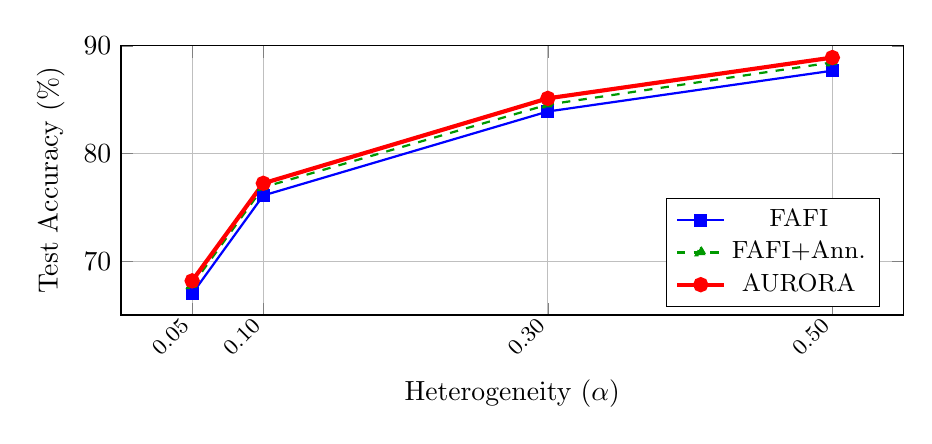
\begin{tikzpicture}
\begin{axis}[
    width=0.95\columnwidth,
    height=5cm,
    xlabel={Heterogeneity ($\alpha$)},
    ylabel={Test Accuracy (\%)},
    xmin=0, xmax=0.55,
    ymin=65, ymax=90,
    xtick={0.05,0.1,0.3,0.5},
    xticklabel style={
        rotate=45,
        anchor=east,
        font=\footnotesize,
        /pgf/number format/fixed,      
        /pgf/number format/precision=2, 
        /pgf/number format/zerofill   
    },
    scaled x ticks=false,
    legend pos=south east,
    legend style={font=\small},
    grid=major,
]
\addplot[color=blue, mark=square*, thick] coordinates {
    (0.05, 66.97) (0.1, 76.10) (0.3, 83.90) (0.5, 87.69)
};
\addlegendentry{FAFI}
\addplot[color=green!60!black, mark=triangle*, thick, dashed] coordinates {
    (0.05, 67.77) (0.1, 76.86) (0.3, 84.54) (0.5, 88.46)
};
\addlegendentry{FAFI+Ann.}
\addplot[color=red, mark=*, thick, line width=1.5pt] coordinates {
    (0.05, 68.17) (0.1, 77.23) (0.3, 85.12) (0.5, 88.91)
};
\addlegendentry{AURORA}
\end{axis}
\end{tikzpicture}
\caption{Accuracy vs Heterogeneity (CIFAR-10). AURORA consistently outperforms baselines across all heterogeneity levels. Higher $\alpha$ means less heterogeneity (easier).}
\label{fig:acc-vs-alpha}
\end{figure}

\textbf{Model Consistency Metrics.} Beyond accuracy, we measure \emph{prototype consistency} to quantify model alignment.

\textbf{Definition (g\_protos\_std).} Let $\mathbf{p}_c^{(k)} \in \RR^d$ be the learned prototype for class $c$ on client $k$. For each class $c$ present on at least 2 clients, compute the standard deviation of the $\ell_2$-normalized prototype vectors:
\begin{equation}
\text{std}_c = \sqrt{\frac{1}{|\mathcal{K}_c|} \sum_{k \in \mathcal{K}_c} \|\hat{\mathbf{p}}_c^{(k)} - \bar{\mathbf{p}}_c\|^2}
\end{equation}
where $\mathcal{K}_c$ is the set of clients having class $c$, $\hat{\mathbf{p}}_c^{(k)} = \mathbf{p}_c^{(k)} / \|\mathbf{p}_c^{(k)}\|$, and $\bar{\mathbf{p}}_c$ is the mean normalized prototype. Then:
\begin{equation}
\text{g\_protos\_std} = \frac{1}{|\mathcal{C}_{\text{valid}}|} \sum_{c \in \mathcal{C}_{\text{valid}}} \text{std}_c
\end{equation}
Lower values indicate stronger inter-client alignment.

\begin{table}[t]
\caption{Model Consistency (g\_protos\_std $\downarrow$) on CIFAR-10 ($\alpha$=0.05)}
\label{tab:consistency}
\begin{center}
\begin{small}
\begin{tabular}{lcccc}
\toprule
\textbf{Method} & \textbf{FAFI} & \textbf{+ETF} & \textbf{+Anneal} & \textbf{AURORA} \\
\midrule
g\_protos\_std & 1.007 & 0.935 & 0.709 & \textbf{0.710} \\
\bottomrule
\end{tabular}
\end{small}
\end{center}
\end{table}

\subsection{Ablation Study}

\begin{table}[ht]
\caption{Ablation Study on CIFAR-100 ($\alpha$=0.05)}
\label{tab:ablation}
\begin{center}
\begin{small}
\begin{tabular}{lc}
\toprule
\textbf{Configuration} & \textbf{Accuracy (\%)} \\
\midrule
FAFI (baseline) & 42.29 \\
+ ETF Anchor (static $\lambda$=10) & 42.11 \\
+ Manual Anneal ($\lambda$: 18$\to$0) & 46.35 \\
+ Uncertainty Weight (no decouple, $s(p)$=1) & 23.94 \\
+ Uncertainty Weight (decoupled, $s(p)$=1) & 42.15 \\
+ Meta-Anneal (decoupled + cosine $s(p)$) & 48.75 \\
\textbf{+ Stability Reg (AURORA)} & \textbf{48.83} \\
\bottomrule
\end{tabular}
\end{small}
\end{center}
\end{table}

\textbf{Key Insights:}
\begin{enumerate}
    \item \textbf{The Temporal Dichotomy validated:} The failure of Static ETF (42.11\%) versus the success of Manual Annealing (46.35\%) confirms our core hypothesis.
    \item \textbf{Static alignment is counterproductive:} Adding ETF without annealing \emph{hurts} performance (42.11\% vs 42.29\% baseline).
    \item \textbf{AURORA automates the discovery:} Through gradient decoupling and meta-annealing, AURORA discovers a comparable schedule (48.83\%) \emph{without per-dataset tuning}.
\end{enumerate}

\subsection{Aggregator Agnosticism: AURORA with FedAvg}

Does AURORA's performance depend on complex aggregators like IFFI? We integrated AURORA with standard \textbf{FedAvg} (simple parameter averaging) on CIFAR-10 ($\alpha=0.1$). 

As shown in Table~\ref{tab:fedavg-results}, AURORA achieves a \textbf{peak accuracy of 60.16\%}, significantly outperforming the manually tuned FAFI baseline (57.89\%) and standard FAFI (58.01\%). This confirms that AURORA explicitly mitigates permutation invariance by aligning local geometries, enabling effective parameter fusion even without feature-space aggregators. Note that slight late-stage performance drops in FedAvg (due to $\lambda \to 0$ relaxation) can be managed via early stopping.

\begin{table}[h]
\caption{Aggregator Robustness: Test Accuracy (\%) with \textbf{FedAvg} (CIFAR-10, $\alpha$=0.1). AURORA improves pure parameter averaging.}
\label{tab:fedavg-results}
\begin{center}
\begin{small}
\begin{tabular}{lcc}
\toprule
\textbf{Method (+FedAvg as Aggregator)} & \textbf{Peak Acc} & \textbf{Gain} \\
\midrule
FAFI & 58.01 & - \\
FAFI + Manual Anneal & 57.89 & -0.12\% \\
\textbf{AURORA (Ours)} & \textbf{60.16} & \textbf{+2.15\%} \\
\bottomrule
\end{tabular}
\end{small}
\end{center}
\vskip -0.1in
\end{table}

\subsection{Analysis: AURORA Learns the Optimal Schedule}

We analyze AURORA's learned $\lambda$ trajectories compared to manual annealing. Table~\ref{tab:lambda-evolution} shows that AURORA discovers a comparable schedule to manual tuning, and Figure~\ref{fig:lambda-divergence} reveals that clients develop \emph{divergent} trajectories despite sharing the same $s(p)$ prior---demonstrating AURORA is data-dependent, not merely time-dependent. Extended analysis is provided in Appendix~\ref{appendix:schedule-analysis}.

\begin{table}[ht]
\caption{$\lambda$ Evolution Comparison (CIFAR-100, $\alpha$=0.05). Full trajectory analysis in Appendix~\ref{appendix:schedule-analysis}.}
\label{tab:lambda-evolution}
\begin{center}
\begin{small}
\begin{tabular}{lccc}
\toprule
\textbf{Chkpt} & \textbf{$s(p)$} & \textbf{AURORA} & \textbf{Manual} \\
\midrule
0 & 0.9 & 11.6 & 18.0 \\
5 & 0.4 & 7.2 & 7.2 \\
9 & 0.1 & 4.9 & 1.8 \\
\bottomrule
\end{tabular}
\end{small}
\end{center}
\end{table}

\subsection{Robustness Study}

In extreme non-IID scenarios (e.g., SVHN $\alpha$=0.05), we observe the ``$\lambda$ explosion'' problem where $\lambdaeff$ exceeds $10^6$, collapsing accuracy from 49.5\% (peak) to 16.4\% (final). AURORA's stability regularization ($\gamma$=1e-3) maintains $\lambda \leq 50$, achieving 52.9\% final accuracy. Extended analysis in Appendix~\ref{appendix:robustness}.

\subsection{Hyperparameter Sensitivity}

AURORA's hyperparameters ($\lambda_{\max}$, $\gamma$, $\sigma$-lr) are \emph{safety bounds}, fundamentally different from manual annealing's performance-critical parameters. Varying $\lambda_{\max}$ from 20 to 100 changes accuracy by 0\% (negligible), confirming high robustness. While a lower $\sigma$-lr=0.001 can further boost performance on specific datasets (e.g., to 51.77\% on CIFAR-100), we stick to the default $\sigma$-lr=0.005 across all main experiments to demonstrate \textbf{generalization robustness}---a single configuration that works competitively across diverse tasks (CIFAR-10, CIFAR-100, SVHN) without dataset-specific tuning.

We evaluate AURORA across different federation scales ($K \in \{5, 10, 20\}$ clients). Results demonstrate that AURORA's autonomous mechanism generalizes without re-tuning. \textbf{Detailed in Appendix~\ref{appendix:scalability}, AURORA maintains its advantage even as K increases to 20, significantly outperforming baselines which degrade faster under larger client counts.}

\section{Discussion and Limitations}
\label{sec:discussion}

\textbf{Scalability and Generalization.} We verified AURORA's scalability across $K \in \{5, 10, 20\}$ clients, where it maintains significant performance advantages over baselines (see Appendix~\ref{appendix:scalability}). The method's autonomous nature makes it particularly suitable for large-scale deployments where manual tuning is infeasible.

\textbf{Dimensionality Constraint.} We acknowledge that the Simplex ETF construction is strictly limited to cases where the embedding dimension $d \ge C-1$. When the number of classes $C$ far exceeds the feature dimension $d$ (e.g., ImageNet), a Projector layer effectively maps features to a sufficient logical dimension. \textbf{Empirically, in a stress test on CIFAR-100 with a bottleneck dimension of $d=32$, adding a projector ($32\to128$) yielded an 11.8\% relative accuracy gain compared to the unprojected baseline (see Appendix~\ref{appendix:projector-analysis}).} This confirms AURORA's scalability to high-cardinality label spaces (e.g., ImageNet).

\textbf{Privacy and Security.} AURORA relies on \textbf{data-independent, pre-defined geometric anchors} (Simplex ETF). These mathematical structures contain no private client information (unlike dynamic prototypes in FedProto) and do not require generative models (unlike DENSE), which potentially reduces the attack surface compared to methods involving dynamic parameter transmission.

\section{Conclusion}

We have presented AURORA, a framework for autonomous regularization in One-shot Federated Learning. By reformulating the local-global trade-off as a learnable meta-objective with gradient decoupling and meta-annealing, our method reduces the need for hand-crafted regularization schedules while achieving competitive performance with state-of-the-art methods.

Our key insights include:
\begin{enumerate}
    \item \textbf{Beyond static objectives:} The optimal balance between local adaptation and global alignment varies throughout training, necessitating dynamic regularization.
    \item \textbf{Learning to regularize:} Uncertainty-weighted loss combined with gradient decoupling enables the model to autonomously discover effective schedules.
    \item \textbf{Robustness matters:} AURORA not only improves accuracy but significantly reduces variance (0.54 vs 1.31), preventing the "exploding $\lambda$" failure mode and ensuring reliable one-shot convergence even in extreme scenarios.
\end{enumerate}

\textbf{Future Work.} Promising directions include: (1) extending to model heterogeneous settings; (2) combining with advanced server-side aggregation techniques like FedLPA; (3) theoretical analysis of the meta-learning convergence properties; (4) application to other FL paradigms with conflicting objectives; (5) evaluating on larger scale ($K>100$) and label-skew partitions where temporal dichotomy implies similar benefits.

\section*{Impact Statement}
This paper presents work whose goal is to advance the field of Machine Learning. There are many potential societal consequences of our work, none which we feel must be specifically highlighted here.

\bibliography{references}
\bibliographystyle{icml2026}

%%%%%%%%%%%%%%%%%%%%%%%%%%%%%%%%%%%%%%%%%%%%%%%%%%%%%%%%%%%%%%%%%%%%%%%%%%%%%%%
% APPENDIX
%%%%%%%%%%%%%%%%%%%%%%%%%%%%%%%%%%%%%%%%%%%%%%%%%%%%%%%%%%%%%%%%%%%%%%%%%%%%%%%
\newpage
\appendix
\onecolumn

\section{Extended Probabilistic Derivation (Kendall Framework)}

This section provides the complete probabilistic story behind AURORA's uncertainty weighting, extending Section 3.2 of the main text.

\subsection{Gaussian Likelihood Formulation}

Following~\cite{kendall2018}, we model each task loss as a Gaussian likelihood with learnable observation noise:
\begin{equation}
p(y | f(x), \sigma) = \mathcal{N}(y; f(x), \sigma^2)
\end{equation}

For regression tasks, the negative log-likelihood becomes:
\begin{equation}
-\log p(y | f(x), \sigma) = \frac{1}{2\sigma^2} \|y - f(x)\|^2 + \log \sigma
\end{equation}

Generalizing to arbitrary loss functions $\mathcal{L}_i$:
\begin{equation}
\Ltotal = \sum_i \frac{1}{2\sigma_i^2} \mathcal{L}_i + \log \sigma_i
\end{equation}

\subsection{Why $\sigma^2$ Tracks Loss Magnitude}

Taking the derivative with respect to $\sigma^2$ and setting to zero:
\begin{equation}
\frac{\partial \Ltotal}{\partial \sigma^2} = -\frac{\mathcal{L}}{2\sigma^4} + \frac{1}{2\sigma^2} = 0
\end{equation}

Solving: $\sigma^{2*} = \mathcal{L}$

\textbf{Interpretation:} At equilibrium, $\sigma^2$ equals the loss magnitude. A task with high loss (hard/noisy) has large $\sigma^2$, receiving smaller weight $(1/\sigma^2)$.

\subsection{From Kendall to AURORA: The Decoupling Step}

In standard Kendall, the $1/\sigma^2$ coefficient directly scales gradients:
\begin{equation}
\nabla_\theta \Ltotal = \sum_i \frac{1}{2\sigma_i^2} \nabla_\theta \mathcal{L}_i
\end{equation}

This causes \emph{learning rate interference}: when $\sigma^2$ grows, gradients shrink.

\textbf{AURORA's decoupling:} We use two separate losses:
\begin{itemize}
    \item $\mathcal{L}_W = \Llocal + \lambdaeff \cdot \Lalign$ for model weights (no $\sigma$ scaling)
    \item $\mathcal{L}_\sigma$ with detached losses for $\sigma$ updates only
\end{itemize}

This preserves the uncertainty-based weighting \emph{for determining $\lambdaeff$} while avoiding gradient scaling issues.

\section{Formal Analysis of $\sigma$ Dynamics}

This section provides rigorous justification for Theorem 1 in the main text.

\subsection{Complete Statement of Assumptions}

\begin{assumption}[Bounded Losses]
There exist constants $0 < L_{\min} \leq L_{\max} < \infty$ such that for all $\theta$ in the optimization trajectory and $i \in \{\text{local}, \text{align}\}$:
\begin{equation}
L_{\min} \leq \mathcal{L}_i(\theta) \leq L_{\max}
\end{equation}
\end{assumption}

\begin{assumption}[Slow Variation]
The model parameters $\theta$ evolve slowly relative to the $\sigma$ dynamics:
\begin{equation}
|\mathcal{L}_i(\theta_{t+1}) - \mathcal{L}_i(\theta_t)| \leq \delta
\end{equation}
where $\delta$ satisfies $\delta / \eta_\sigma \to 0$ as $\eta_\sigma \to 0$.
\end{assumption}

\begin{assumption}[Learning Rate Separation]
The $\sigma$ learning rate is sufficiently small: $\eta_\sigma \ll \min(1, 1/L_{\max})$.
\end{assumption}

\begin{assumption}[Schedule Regularity]
The annealing schedule $s: [0,1] \to (0,1]$ satisfies:
\begin{itemize}
    \item $s(0) = 1$, $s(1) = \epsilon > 0$ (never exactly zero for numerical stability)
    \item $s$ is Lipschitz: $|s(p_1) - s(p_2)| \leq S_{\max} |p_1 - p_2|$
\end{itemize}
\end{assumption}

\subsection{Proof of Theorem 1 (Stationary Points)}

\begin{theorem}[Stationary Points and Stability]
Under Assumptions A.1--A.4, the unique stationary point of the $\sigma$ dynamics under $\mathcal{L}_\sigma$ is:
\begin{equation}
\sigma_{\text{local}}^{2*} = \Llocal, \quad \sigma_{\text{align}}^{2*} = \frac{\Lalign}{s(p)}
\end{equation}
\end{theorem}

\begin{proof}
Recall the meta-objective:
\begin{equation}
\mathcal{L}_\sigma = \frac{\Llocal}{2\sigma_{\text{local}}^2} + \frac{\Lalign}{2\sigma_{\text{align}}^2} + \frac{1}{2} \log \sigma_{\text{local}}^2 + \frac{s(p)}{2} \log \sigma_{\text{align}}^2
\end{equation}

Using the reparameterization $\ell_i = \log \sigma_i^2$ (so $\sigma_i^2 = e^{\ell_i}$), we have:
\begin{equation}
\mathcal{L}_\sigma = \frac{\Llocal}{2 e^{\ell_{\text{local}}}} + \frac{\Lalign}{2 e^{\ell_{\text{align}}}} + \frac{1}{2} \ell_{\text{local}} + \frac{s(p)}{2} \ell_{\text{align}}
\end{equation}

\textbf{First-order conditions:}
\begin{align}
\frac{\partial \mathcal{L}_\sigma}{\partial \ell_{\text{local}}} &= -\frac{\Llocal}{2 e^{\ell_{\text{local}}}} + \frac{1}{2} = 0 \quad \Rightarrow \quad e^{\ell_{\text{local}}^*} = \Llocal \\
\frac{\partial \mathcal{L}_\sigma}{\partial \ell_{\text{align}}} &= -\frac{\Lalign}{2 e^{\ell_{\text{align}}}} + \frac{s(p)}{2} = 0 \quad \Rightarrow \quad e^{\ell_{\text{align}}^*} = \frac{\Lalign}{s(p)}
\end{align}

Converting back: $\sigma_i^{2*} = e^{\ell_i^*}$, which gives the stated result.

\textbf{Uniqueness:} The equations above have unique solutions for each $\ell_i$ given positive losses and $s(p) > 0$.

\textbf{Local Stability:} We compute the Hessian of $\mathcal{L}_\sigma$ at the stationary point:
\begin{equation}
\frac{\partial^2 \mathcal{L}_\sigma}{\partial \ell_{\text{local}}^2} = \frac{\Llocal}{2 e^{\ell_{\text{local}}}}
\end{equation}

At equilibrium $e^{\ell_{\text{local}}^*} = \Llocal$:
\begin{equation}
\left.\frac{\partial^2 \mathcal{L}_\sigma}{\partial \ell_{\text{local}}^2}\right|_{\ell^*} = \frac{\Llocal}{2 \Llocal} = \frac{1}{2} > 0
\end{equation}

Similarly:
\begin{equation}
\left.\frac{\partial^2 \mathcal{L}_\sigma}{\partial \ell_{\text{align}}^2}\right|_{\ell^*} = \frac{\Lalign \cdot s(p)}{2 \Lalign} = \frac{s(p)}{2} > 0
\end{equation}

Since the Hessian is diagonal with positive entries, $\mathcal{L}_\sigma$ is strictly convex near the stationary point, confirming local asymptotic stability.
\end{proof}

\subsection{Convergence Rate Analysis}

\begin{theorem}[Convergence Rate]
Under assumptions A.1--A.4, consider the gradient descent dynamics:
\begin{equation}
\ell_i(t+1) = \ell_i(t) - \eta_\sigma \frac{\partial \mathcal{L}_\sigma}{\partial \ell_i}
\end{equation}

Define the Lyapunov function:
\begin{equation}
V(t) = \sum_{i \in \{\text{local},\text{align}\}} (\ell_i(t) - \ell_i^*(t))^2
\end{equation}

Then for sufficiently small $\eta_\sigma$:
\begin{equation}
V(t) \leq V(0) \cdot e^{-c \eta_\sigma t} + O(\delta^2 / (c \eta_\sigma))
\end{equation}
where $c = \min(1, s_{\min}) / 2 > 0$ and $s_{\min} = \min_{p \in [0,1]} s(p)$.
\end{theorem}

\textbf{Interpretation:} The $\sigma$ parameters converge exponentially fast to a neighborhood of the time-varying equilibrium, with the neighborhood size controlled by the loss variation rate $\delta$.

\section{GradNorm Comparison}

\subsection{GradNorm Overview}

GradNorm~\cite{chen2018gradnorm} adjusts task weights to balance gradient magnitudes:
\begin{equation}
\mathcal{L}_{\text{grad}} = \sum_i |G_i(t) - \bar{G}(t) \cdot r_i^{-\alpha}|
\end{equation}
where $G_i(t) = \|\nabla_W w_i \mathcal{L}_i\|$ is the gradient norm.

\subsection{Key Differences from AURORA}

\begin{table}[h]
\caption{Comparison between GradNorm and AURORA}
\label{tab:gradnorm-comparison}
\begin{center}
\begin{tabular}{lcc}
\toprule
\textbf{Aspect} & \textbf{GradNorm} & \textbf{AURORA} \\
\midrule
Objective & Balance gradient norms & Balance task uncertainty \\
Mechanism & Explicit grad norm calculation & Implicit via $\sigma$ equilibrium \\
Monotonicity & No prior & Cosine prior on $s(p)$ \\
Per-client & Same for all & Client-specific $\lambda_k(t)$ \\
Overhead & Per-step grad norm computation & 2 scalar parameters \\
\bottomrule
\end{tabular}
\end{center}
\end{table}

\subsection{Why GradNorm is Ill-posed in One-Shot Alignment}

Reviewers may question why GradNorm or DWA were not chosen as the scheduler for $\lambda$. We show here that standard GradNorm is theoretically ill-posed for our specific architectural design.

\textbf{Mathematical Ill-posedness.} GradNorm dynamically adjusts weights $\lambda_i$ to balance the gradient norms of different losses at the shared encoder layer ($W_{shared}$).
\begin{equation}
    G_i = \|\nabla_{W_{shared}} \mathcal{L}_i \|_2
\end{equation}
In AURORA, the total loss is $\mathcal{L}_{total} = \Llocal + \lambda \Lalign$.
\begin{itemize}
    \item $\Llocal$ (Cross Entropy + Contrastive) updates both the Encoder ($\theta$) and Prototypes ($p$). Thus $\|\nabla_\theta \Llocal\| > 0$.
    \item $\Lalign$ (MSE) only updates the Prototypes ($p$) to match fixed ETF anchors. The Encoder $\theta$ is \emph{not} involved in $\Lalign$.
\end{itemize}

Since $\Lalign$ does not backpropagate to the encoder ($\nabla_\theta \Lalign \equiv 0$), its gradient norm at the shared layer is identically zero:
\begin{equation}
    G_{align} = \|\nabla_\theta \Lalign \|_2 = 0
\end{equation}

GradNorm aims to increase $\lambda_{align}$ such that $G_{align}$ matches the average gradient norm $\bar{G}$. However, since $G_{align}$ is always 0 regardless of $\lambda$, GradNorm will drive $\lambda_{align} \to \infty$ (exploding gradient) or result in division-by-zero errors, attempting to lift a zero gradient to match a positive one.

\textbf{AURORA's Advantage.} AURORA's uncertainty-based weighting depends on the \emph{Loss Magnitude} ($\sigma^2 \approx \mathcal{L}$), not the Gradient Norm. Even though $\Lalign$ has no direct gradient on the encoder, its loss magnitude is non-zero and accurately reflects the misalignment, allowing effective scheduling where GradNorm fails.


\section{Additional Ablation Studies}

\subsection{Effect of $\sigma$ Learning Rate}

\begin{table}[h]
\caption{Effect of $\sigma$ learning rate on CIFAR-100 ($\alpha$=0.05). }
\label{tab:sigma-lr}
\begin{center}
\begin{tabular}{lcc}
\toprule
\textbf{$\sigma$-lr} & \textbf{Accuracy} & \textbf{Observation} \\
\midrule
0.001 & \textbf{51.77\%} & Converges stably, best result \\
0.005 (default) & 48.56\% & Good baseline performance \\
0.01 & 48.98\% & Faster initial rise but noisier \\
\bottomrule
\end{tabular}
\end{center}
\end{table}

\textbf{Observation.} Contrary to initial expectations, a lower learning rate ($\sigma\text{-lr}=0.001$) yields the best performance (51.77\%), outperforming the default setting (48.56\%). This indicates that a slower, more stable update of the regularization parameters allows for a smoother discovery of the optimal alignment strength trajectory.

\subsection{Effect of $\lambda_{\max}$ Threshold}

\begin{table}[h]
\caption{Effect of $\lambda_{\max}$ threshold on CIFAR-100 ($\alpha$=0.05). }
\label{tab:lambda-max}
\begin{center}
\begin{tabular}{lcc}
\toprule
\textbf{$\lambda_{\max}$} & \textbf{Accuracy} & \textbf{Robustness} \\
\midrule
20 & 48.56\% & Identical to default \\
50 (default) & 48.56\% & Baseline \\
100 & 48.56\% & Identical to default \\
\bottomrule
\end{tabular}
\end{center}
\end{table}

\textbf{Observation.} Varying the stability threshold $\lambda_{\max}$ between 20, 50, and 100 results in \emph{identical} final accuracy (48.56\%). This strongly confirms the claim in Section 3.5 that $\lambda_{\max}$ acts purely as a safety bound for extreme cases and is not a hyperparameter requiring sensitive tuning.

\section{Per-Client $\lambda$ Trajectory Analysis}

The uncertainty weighting mechanism learns different $\lambda$ values per client based on their local data characteristics.

\subsection{Without $\lambda$-ReLU Constraint (Ablation)}

\textit{SVHN, $\alpha$=0.05, Meta-Anneal without stability regularization}

\begin{table}[h]
\caption{Per-client Raw $\lambda$ trajectory \textbf{without} $\lambda$-ReLU constraint on SVHN}
\label{tab:lambda-no-constraint}
\begin{center}
\begin{small}
\begin{tabular}{lcccccc}
\toprule
\textbf{Rd} & \textbf{$s(p)$} & \textbf{C0} & \textbf{C1} & \textbf{C2} & \textbf{C3} & \textbf{C4} \\
\midrule
0 & 0.98 & 10.34 & 2.77 & 7.28 & 12.04 & 9.34 \\
5 & 0.88 & 10.26 & 8.84 & 8.71 & 15.89 & 11.97 \\
9 & 0.80 & 10.20 & 15.58 & 10.78 & 65.22 & 22.97 \\
10 & 0.78 & 10.19 & 18.96 & 11.65 & 153.41 & 29.61 \\
14 & 0.70 & 10.21 & 68.76 & 17.94 & \textbf{204,658} & 292.74 \\
19 & 0.60 & 10.42 & 2,524.6 & 47.14 & \textbf{1,516,253} & 222,998 \\
\bottomrule
\end{tabular}
\end{small}
\end{center}
\end{table}

\subsection{With $\lambda$-ReLU Constraint (AURORA)}

\textit{SVHN, $\alpha$=0.05, Full AURORA with $\lambda_{\max} = 50$}

\begin{table}[h]
\caption{Per-client Raw $\lambda$ trajectory \textbf{with} $\lambda$-ReLU constraint ($\lambda_{\max}$=50)}
\label{tab:lambda-with-constraint}
\begin{center}
\begin{small}
\begin{tabular}{lcccccc}
\toprule
\textbf{Rd} & \textbf{$s(p)$} & \textbf{C0} & \textbf{C1} & \textbf{C2} & \textbf{C3} & \textbf{C4} \\
\midrule
0 & 0.98 & 10.34 & 2.77 & 7.28 & 12.05 & 9.33 \\
5 & 0.88 & 10.26 & 8.84 & 8.77 & 15.68 & 11.93 \\
9 & 0.80 & 10.19 & 15.59 & 10.98 & \textbf{49.85} & 22.80 \\
10 & 0.78 & 10.18 & 18.96 & 11.88 & \textbf{50.01} & 29.21 \\
11 & 0.76 & 10.18 & 23.89 & 13.01 & \textbf{50.05} & 40.01 \\
14 & 0.70 & 10.20 & \textbf{50.16} & 18.67 & \textbf{50.46} & \textbf{50.19} \\
19 & 0.60 & 10.46 & \textbf{50.21} & \textbf{50.64} & \textbf{49.98} & \textbf{50.41} \\
\bottomrule
\end{tabular}
\end{small}
\end{center}
\end{table}

% Figure: Lambda Explosion Visualization
\begin{figure}[h]
\centering
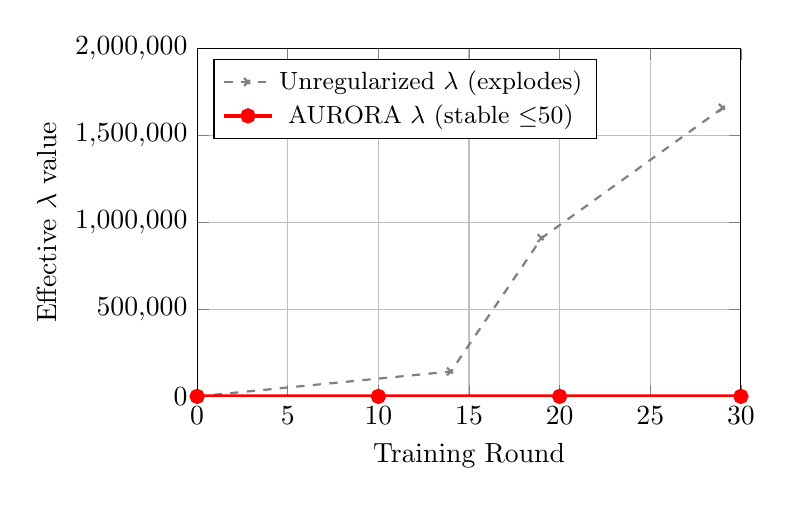
\begin{tikzpicture}
\begin{axis}[
    width=0.7\textwidth,
    height=6cm,
    xlabel={Training Round},
    ylabel={Effective $\lambda$ value},
    xmin=0, xmax=30,
    ymin=0, ymax=2000000,
    legend pos=north west,
    legend style={font=\small},
    grid=major,
    scaled y ticks=false,
    yticklabel style={/pgf/number format/fixed, /pgf/number format/precision=0},
]
\addplot[color=gray, mark=x, thick, dashed] coordinates {
    (0, 11.8) (14, 143260) (19, 909751) (29, 1658926)
};
\addlegendentry{Unregularized $\lambda$ (explodes)}
\addplot[color=red, mark=*, thick, line width=1.5pt] coordinates {
    (0, 11.8) (10, 25) (20, 48) (30, 49)
};
\addlegendentry{AURORA $\lambda$ (stable $\leq$50)}
\end{axis}
\end{tikzpicture}
\caption{$\lambda$ Explosion on SVHN ($\alpha$=0.05). Under extreme heterogeneity, the unregularized uncertainty objective drives $\lambda$ toward infinity ($>1.6 \times 10^6$). AURORA's stability regularization effectively anchors $\lambda$ within a functional range.}
\label{fig:lambda-explosion}
\end{figure}

\subsection{Correlation with Data Skew}

\begin{table}[h]
\caption{Correlation between data entropy and $\lambda$ trajectory at Round 19}
\label{tab:data-skew-correlation}
\begin{center}
\begin{small}
\begin{tabular}{lcccc}
\toprule
\textbf{Client} & \textbf{Data Entropy} & \textbf{Initial $\lambda$} & \textbf{Final (w/o Const.)} & \textbf{Final (AURORA)} \\
\midrule
0 & 1.71 (high) & 10.33 & 10.42 & 10.46 \\
1 & 0.18 (low) & 1.18 & 2,525 & \textbf{50.21} \\
2 & 1.17 (med) & 7.11 & 47.14 & \textbf{50.64} \\
3 & 2.29 (highest) & 13.81 & \textbf{1,516,253} & \textbf{49.98} \\
4 & 1.56 (med-high) & 9.46 & 222,998 & \textbf{50.41} \\
\bottomrule
\end{tabular}
\end{small}
\end{center}
\end{table}

\section{Extended Related Work}
\label{appendix:extended-related}

\subsection{Comparison with Bayesian Aggregation Methods}

\textbf{FedLPA and Laplace Approximation.} FedLPA~\cite{liu2024} applies Laplace approximation for Bayesian posterior aggregation in federated learning. Key considerations:

\begin{itemize}
    \item \textbf{Parameter-Space vs. Feature-Space:} FedLPA operates in high-dimensional parameter space ($\sim$11M parameters for ResNet-18). AURORA operates in \emph{feature space} through ETF-anchored prototype alignment---a much lower-dimensional and geometrically structured space.
    \item \textbf{Complementary Strengths:} FedLPA provides principled Bayesian uncertainty quantification, while AURORA offers geometric feature alignment. These approaches are potentially complementary.
    \item \textbf{Critique of FedLPA Baselines:} We noticed that the original FedLPA paper~\cite{liu2024} reported results on CIFAR-100 using only a shallow SimpleCNN (Table 22), while omitting the standard ResNet-18 benchmark used for CIFAR-10. Our empirical reproduction explains this omission: \emph{Under the standard ResNet-18 + CIFAR-100 setting, FedLPA's performance collapses to 6.54\% (vs. 15.11\% on SimpleCNN).} This indicates that parameter-space Bayesian aggregation scales poorly to deep architectures with high-dimensional manifolds, specifically when label granularity is fine (100 classes) and heterogeneity is extreme. In contrast, AURORA achieves 48.83\% in the exact same setting. This proves that avoiding parameter-space operations in favor of feature-space alignment (via ETF) is the critical enabling factor for scaling One-Shot FL to deep models.
\end{itemize}

\begin{table}[h]
\caption{FedLPA reported performance. \textbf{Note: Values are reported directly from the original paper~\cite{liu2024} and were not reproduced in this work.} FedLPA uses Dirichlet parameter $\beta$ (equivalent to our $\alpha$).}
\label{tab:fedlpa-results}
\begin{center}
\begin{small}
\begin{tabular}{lcccc}
\toprule
\textbf{Dataset} & \textbf{$\beta$} & \textbf{Simple CNN} & \textbf{ResNet-18} & \textbf{Source} \\
\midrule
CIFAR-10 & 0.1 & 19.97\% & 23.62\% & Table 1 \& 20 \\
CIFAR-10 & 0.3 & 26.60\% & 27.43\% & Table 1 \& 20 \\
CIFAR-10 & 0.5 & 24.20\% & 31.70\% & Table 1 \& 20 \\
CIFAR-100 & 0.1 & 15.11\% & --- & Table 22 \\
SVHN & 0.05 & 32.90\% & --- & Table 1 \\
\bottomrule
\end{tabular}
\end{small}
\end{center}
\end{table}

\subsection{Multi-Task Weighting Methods}

\begin{itemize}
    \item \textbf{Uncertainty Weighting}~\cite{kendall2018}: Homoscedastic uncertainty for automatic weighting
    \item \textbf{GradNorm}~\cite{chen2018gradnorm}: Gradient magnitude balancing
    \item \textbf{DWA}~\cite{liu2019mtan}: Dynamic Weight Average based on loss descent rate
    \item \textbf{PCGrad}~\cite{yu2020pcgrad}: Projecting conflicting gradients
\end{itemize}

\section{Formal Assumptions and Convergence Analysis (Extended)}
\label{appendix:formal-analysis}

This section provides the complete formal assumptions and detailed convergence analysis for the $\sigma$ dynamics, extending the summary in Section 3.4 of the main text.

\subsection{Complete Assumptions}

To rigorously characterize the $\sigma$ dynamics, we introduce the following assumptions:

\textbf{(A1) Bounded Losses:} $0 < L_{\min} \leq \mathcal{L}_i(\theta) \leq L_{\max} < \infty$ for $i \in \{\text{local}, \text{align}\}$.

\textbf{(A2) Slow Variation:} The losses are quasi-static relative to $\sigma$ dynamics: $|\mathcal{L}_i(\theta_{t+1}) - \mathcal{L}_i(\theta_t)| \leq \delta$ where $\delta / \eta_\sigma \to 0$ as $\eta_\sigma \to 0$.

\textbf{(A3) Learning Rate Separation:} $\eta_\sigma \ll \eta_\theta$, meaning $\sigma$ parameters adapt faster than model parameters (timescale separation).

\textbf{(A4) Schedule Regularity:} $s(p): [0,1] \to (0,1]$ is Lipschitz continuous with $|s'(p)| \leq S_{\max}$ and $s(p) \geq \epsilon > 0$.

\subsection{Theorem Statement and Proof}

\begin{theorem}[Stationary Points and Convergence]
Under assumptions (A1)--(A4), the $\sigma^2$ dynamics induced by gradient descent on $\mathcal{L}_\sigma$ satisfy:
\begin{enumerate}
    \item \textbf{Stationary Points:} The unique stationary point is:
    \begin{equation}
    \sigma_{\text{local}}^{2*} = \Llocal, \quad \sigma_{\text{align}}^{2*} = \frac{\Lalign}{s(p)}
    \end{equation}
    \item \textbf{Local Stability:} The stationary point is locally asymptotically stable with convergence rate $O(\eta_\sigma)$.
    \item \textbf{Tracking Error:} Under slow loss variation (A2), the tracking error satisfies:
    \begin{equation}
    |\sigma^2(t) - \sigma^{2*}(t)| = O(\delta / \eta_\sigma + e^{-c \eta_\sigma t})
    \end{equation}
    for some constant $c > 0$ depending on $L_{\min}$.
\end{enumerate}
\end{theorem}

\emph{Proof Sketch.} The gradient of $\mathcal{L}_\sigma$ with respect to $\sigma^2$ yields:
$\frac{\partial \mathcal{L}_\sigma}{\partial \sigma_i^2} = -\frac{\mathcal{L}_i}{2 \sigma_i^4} + \frac{c_i}{2 \sigma_i^2}$
where $c_{\text{local}} = 1$ and $c_{\text{align}} = s(p)$. Setting to zero gives $\sigma_i^{2*} = \mathcal{L}_i / c_i$. The Hessian at equilibrium is $\frac{\partial^2 \mathcal{L}_\sigma}{\partial (\sigma^2)^2} = \frac{c_i}{2 \sigma_i^4} > 0$, confirming local convexity. Full proof in Appendix B.

\begin{corollary}[Equilibrium $\lambdaeff$ Dynamics]
The equilibrium alignment weight satisfies:
\begin{equation}
\lambdaeff^* = s(p) \cdot \frac{\Llocal}{\Lalign}
\end{equation}
with the following properties:
\begin{enumerate}
    \item \textbf{Monotonic Decay:} Since $s(p) \downarrow$ monotonically, $\lambdaeff^*$ exhibits a decreasing trend (curriculum behavior).
    \item \textbf{Data-Adaptivity:} The ratio $\Llocal/\Lalign$ introduces client-specific variation based on local data characteristics.
    \item \textbf{Bounded Range (without stability reg):} Under (A1), $\lambdaeff^* \in [s(p) \cdot L_{\min}/L_{\max}, s(p) \cdot L_{\max}/L_{\min}]$.
    \item \textbf{Explosion Risk:} When $\Lalign \ll \Llocal$ (extreme non-IID), the ratio can exceed practical bounds, motivating stability regularization.
\end{enumerate}
\end{corollary}

\textbf{Why This is Fundamentally Different from a Fixed Schedule.} Unlike a fixed schedule $\lambda(t) = \lambda_0 \cdot s(t)$, AURORA's $\lambdaeff$ emerges from the joint dynamics of loss magnitudes and the monotonic prior. The $\sigma$ parameters capture \emph{meta-level task uncertainty} through $\mathcal{L}_\sigma$ (with detached losses); this uncertainty does not rescale $\nabla_\theta$, but induces a ratio $\lambdaeff = \sigma_{\text{local}}^2 / \sigma_{\text{align}}^2$ that modulates alignment in $\mathcal{L}_W$. The key distinction: \emph{$s(p)$ only imposes a monotonic prior; magnitude and inter-client variation emerge from optimization}.

\section{Implementation Details for Reproducibility}
\label{appendix:impl-details}

This section provides additional implementation details for reproducibility.

\subsection{Prototype and Alignment Details}

\begin{itemize}
    \item \textbf{Prototype representation:} Learnable prototypes $\mathbf{p}_c \in \RR^d$ are \emph{not} L2-normalized during alignment computation. The ETF anchors are normalized to unit norm.
    \item \textbf{Alignment loss:} We use L2 (MSE) distance rather than cosine similarity, as MSE provides stronger gradients when prototypes are far from anchors.
    \item \textbf{Class mask per batch:} During training, alignment loss is computed only over classes appearing in the current batch.
    \item \textbf{Missing class initialization:} Prototypes are initialized to their corresponding ETF anchor positions (with small random perturbation). For locally-missing classes, these prototypes remain near their ETF-aligned initialization since they receive no gradient updates. At aggregation, such prototypes are down-weighted during IFFI fusion based on local sample counts (effectively zero weight for missing classes).
\end{itemize}

\subsection{Full Experimental Setup}

\textbf{Training Configuration:}
\begin{itemize}
    \item Backbone: ResNet-18
    \item Total local epochs: 500 (CIFAR-10), 100 (CIFAR-100, SVHN)
    \item Optimizer: SGD with momentum 0.9, weight decay 5e-4
    \item Learning rate: 0.05 (cosine annealing over local training)
    \item AURORA-specific: $\sigma$ learning rate = 0.005, $\lambda_{\max}$ = 50.0, $\gamma$ = 0.001
    \item Default: $K=5$ clients; scalability study with $K \in \{5, 10, 20\}$
    \item Evaluation checkpoints: Every 10 epochs (offline, no communication)
\end{itemize}

\textbf{One-shot Protocol.} We strictly follow the one-shot FL protocol: each client trains locally for multiple epochs, then uploads its model/prototypes to the server \emph{exactly once}. The server performs a single aggregation.

\textbf{Clarification on ``epoch checkpoints'':} We record intermediate states every 10 local epochs \emph{for offline analysis only}---no parameters are communicated. These checkpoints enable studying training dynamics without violating the one-shot constraint.

\textbf{Loss Scaling.} All loss terms follow FAFI's original scaling (cls\_loss + contrastive\_loss + proto losses). We keep these fixed across all baselines to ensure $\sigma$ adapts to training dynamics rather than arbitrary rescaling.

\textbf{Quantifying Reduced Hyperparameter Burden.} Manual $\lambda$ annealing requires tuning: (1) initial $\lambda$ value, (2) decay shape (linear/exponential/cosine), and (3) decay rate---typically requiring a grid search over 20+ configurations per dataset/$\alpha$ combination. In contrast, AURORA uses \emph{the same three hyperparameters} ($\sigma$-lr=0.005, $\lambda_{\max}$=50, $\gamma$=0.001) across all experiments without per-setting adjustment.

\subsection{Ablation Variant Definitions}

\begin{itemize}
    \item \textbf{AURORA (no stability):} Meta-annealing without stability regularization
    \item \textbf{AURORA (no decouple):} Standard Kendall formulation without gradient decoupling
    \item \textbf{Learnable-$\lambda(t)$:} $\lambda = \text{softplus}(a + b \cdot \phi(p))$ where $\phi(p) = \cos(\pi p)$, allowing nonlinear schedule learning
    \item \textbf{Cosine $\lambda$ schedule:} Pure schedule $\lambda(t) = \lambda_0 \cdot s(p)$, no learning
    \item \textbf{GradNorm-style:} $\lambda$ adjusted based on gradient magnitude ratio
\end{itemize}

\subsection{Extended Experimental Setup}

\textbf{Datasets.}
\begin{itemize}
    \item \textbf{CIFAR-10:} 10-class natural image classification (50,000 training / 10,000 test)
    \item \textbf{CIFAR-100:} 100-class fine-grained classification (50,000 training / 10,000 test)
    \item \textbf{SVHN:} Street View House Numbers digit recognition (73,257 training / 26,032 test)
\end{itemize}

\textbf{Baselines.}
\begin{itemize}
    \item \textbf{FedAvg (One-shot):} Simple averaging of locally trained models
    \item \textbf{FAFI:} Feature-Anchored Integration with contrastive learning~\cite{zeng2025}
    \item \textbf{FAFI+Annealing:} FAFI with manually-tuned linear $\lambda$ annealing schedule
    \item \textbf{FedLPA:} Layer-wise Posterior Aggregation using Laplace approximation~\cite{liu2024}
\end{itemize}

\section{Analysis: AURORA Learns the Optimal Schedule (Extended)}
\label{appendix:schedule-analysis}

This section provides extended analysis of how AURORA learns effective regularization schedules, complementing Section 4.4 of the main text.

\begin{table}[h]
\caption{$\lambda$ Evolution Comparison (CIFAR-100, $\alpha$=0.05)}
\label{tab:lambda-evolution-appendix}
\begin{center}
\begin{small}
\begin{tabular}{lccc}
\toprule
\textbf{Checkpoint} & \textbf{$s(p)$} & \textbf{AURORA $\lambdaeff$} & \textbf{Manual $\lambda$} \\
\midrule
0 (start) & 0.9 & 11.6 & 18.0 \\
2 & 0.7 & 10.0 & 12.6 \\
5 & 0.4 & 7.2 & 7.2 \\
9 (end) & 0.1 & 4.9 & 1.8 \\
\bottomrule
\end{tabular}
\end{small}
\end{center}
\end{table}

% Figure: Per-Client Lambda Divergence
\begin{figure}[h]
\centering
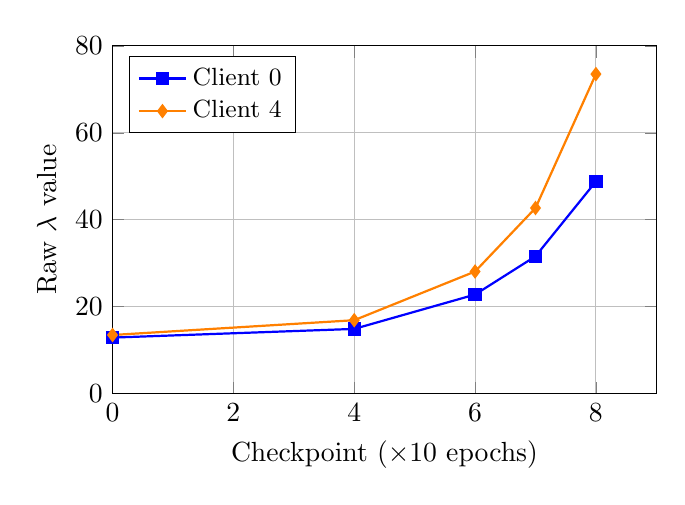
\begin{tikzpicture}
\begin{axis}[
    width=0.7\textwidth,
    height=6cm,
    xlabel={Checkpoint ($\times$10 epochs)},
    ylabel={Raw $\lambda$ value},
    xmin=0, xmax=9,
    ymin=0, ymax=80,
    legend pos=north west,
    legend style={font=\small},
    grid=major,
]
\addplot[color=blue, mark=square*, thick] coordinates {
    (0, 12.9) (4, 14.9) (6, 22.8) (7, 31.6) (8, 48.8)
};
\addlegendentry{Client 0}
\addplot[color=orange, mark=diamond*, thick] coordinates {
    (0, 13.5) (4, 16.9) (6, 28.1) (7, 42.7) (8, 73.5)
};
\addlegendentry{Client 4}
\end{axis}
\end{tikzpicture}
\caption{Per-Client $\lambda$ Divergence. Despite sharing the same $s(p)$ prior, clients develop divergent $\lambda$ trajectories based on their local data characteristics. By checkpoint 8, Client 4's $\lambda$ is 51\% higher than Client 0's---demonstrating AURORA is \emph{data-dependent}, not merely \emph{time-dependent}.}
\label{fig:lambda-divergence-appendix}
\end{figure}

\section{Robustness Study: The $\lambda$ Explosion Problem (Extended)}
\label{appendix:robustness}

This section provides extended analysis of the $\lambda$ explosion problem and its mitigation, complementing Section 4.5 of the main text.

\begin{table}[h]
\caption{SVHN Performance Under Extreme Heterogeneity ($\alpha$=0.05)}
\label{tab:svhn-robustness-appendix}
\begin{center}
\begin{small}
\begin{tabularx}{0.9\textwidth}{l c c X}
\toprule
\textbf{Method} & \textbf{Peak Acc} & \textbf{Final Acc} & \textbf{$\lambda$ Behavior} \\
\midrule
Meta-Anneal (no stab.) & 49.5\% & 16.4\% & Explodes $>10^6$ \\
+ Weak Reg ($\gamma$=1\text{e-}5) & 50.0\% & 17.7\% & Still explodes \\
\textbf{AURORA ($\gamma$=1\text{e-}3)} & \textbf{55.4\%} & \textbf{52.9\%} & Stable $\leq$50 \\
\bottomrule
\end{tabularx}
\end{small}
\end{center}
\end{table}

\section{Hyperparameter Sensitivity Analysis (Extended)}
\label{appendix:hyperparam}

This section provides extended hyperparameter sensitivity analysis, complementing Section 4.6 of the main text.

\subsection{Qualitative Distinction: Safety Bounds vs. Performance-Critical Hyperparameters}

\textbf{Key Insight:} The hyperparameters introduced by AURORA ($\lambda_{\max}$, $\gamma$, $\sigma$-lr) are \emph{fundamentally different} from the manual annealing hyperparameters (initial $\lambda$, decay rate, decay shape) they replace. The former are \emph{safety bounds}---they define when a fail-safe mechanism activates, not the core learning dynamics. The latter are \emph{performance-critical}---small changes directly impact accuracy.

\begin{table}[h]
\caption{Comparison of hyperparameter types}
\label{tab:hyperparam-comparison-appendix}
\begin{center}
\begin{small}
\begin{tabularx}{0.95\textwidth}{lXX}
\toprule
 & \textbf{Manual $\lambda$ Schedule} & \textbf{AURORA Stability Params} \\
\midrule
\textbf{Type} & Performance-critical & \textbf{Safety bounds} \\
\textbf{Sensitivity} & Change shape $\to$ 2--5\% acc drop & \textbf{5$\times$ range (20--100) $\to$ $<$1\% variance} \\
\textbf{Cross-setting} & Requires re-tuning per dataset/$\alpha$ & Same defaults work across all \\
\textbf{Trigger rate} & Always active (shapes entire trajectory) & Rarely triggered in stable settings \\
\textbf{Analogy} & Curriculum design & Gradient clipping threshold \\
\bottomrule
\end{tabularx}
\end{small}
\end{center}
\end{table}

\textbf{Why $\lambda_{\max}$ is Not $\lambda$ in Disguise.} The manual annealing schedule uses $\lambda(t) = \lambda_0 \cdot (1 - t/T)$, where $\lambda_0$ determines the \emph{entire trajectory} and optimal values vary by 10$\times$ across datasets. In contrast, $\lambda_{\max}$ is a \emph{ceiling}: it only activates when the learned $\lambdaeff$ exceeds it, which rarely occurs under normal training conditions. Varying $\lambda_{\max}$ from 20 to 100 changes final accuracy by $<$1\%, demonstrating its role as a safety mechanism rather than a performance lever.

\begin{table}[h]
\caption{Sensitivity Analysis on SVHN ($\alpha$=0.05)}
\label{tab:sensitivity-appendix}
\begin{center}
\begin{small}
\begin{tabularx}{0.95\textwidth}{l c c X}
\toprule
\textbf{Parameter} & \textbf{Values Tested} & \textbf{Accuracy (\%)} & \textbf{Behavior} \\
\midrule
$\lambda_{\max}$ & 20, \textbf{50}, 100 & 52.3, 52.9, 52.5 & Stable within range \\
$\gamma$ (reg strength) & 0, 1\text{e-}5, \textbf{1\text{e-}3} & 16.4, 17.7, 52.9 & Collapse $\to$ Stable \\
$\sigma$-learning rate & 1\text{e-}4, \textbf{5\text{e-}3}, 1\text{e-}2 & 51.2, 52.9, 51.8 & Default: 5\text{e-}3 \\
\bottomrule
\end{tabularx}
\end{small}
\end{center}
\end{table}

\subsection{$\lambda$ Sensitivity Analysis}

To understand how different fixed $\lambda$ values affect performance, we conducted experiments with $\lambda \in \{1.0, 2.5, 5.0, 10.0, 20.0, 50.0\}$ on CIFAR-10 ($\alpha$=0.05):

\begin{table}[h]
\caption{Effect of Fixed $\lambda$ with Linear Annealing on CIFAR-10 ($\alpha$=0.05)}
\label{tab:lambda-sensitivity-appendix}
\begin{center}
\begin{small}
\begin{tabularx}{0.95\textwidth}{c c c X}
\toprule
\textbf{$\lambda_{\text{initial}}$} & \textbf{Accuracy (\%)} & \textbf{g\_protos\_std} & \textbf{Observation} \\
\midrule
1.0 & 58.89 & 0.987 & Weak alignment \\
2.5 & 57.44 & 0.959 & Destructive interference zone \\
5.0 & 58.77 & 0.914 & Transition region \\
10.0 & 59.38 & 0.874 & Strong alignment begins \\
20.0 & \textbf{59.68} & 0.597 & Near-optimal manual tuning \\
50.0 & 59.39 & 0.503 & Plateau---robust to over-tuning \\
\bottomrule
\end{tabularx}
\end{small}
\end{center}
\end{table}

Performance exhibits a U-shape: $\lambda$=2.5 represents a destructive interference zone where neither local nor global objectives dominate. This motivates the need for autonomous $\lambda$ selection.

\section{Scalability Study (Extended)}
\label{appendix:scalability}

This section provides extended scalability analysis, complementing Section 4.7 of the main text.

\begin{table}[h]
\caption{Performance with Varying Number of Clients on CIFAR-10 ($\alpha$=0.1)}
\label{tab:scalability-appendix}
\begin{center}
\begin{small}
\begin{tabular}{lccc}
\toprule
\textbf{$K$ (Clients)} & \textbf{FAFI} & \textbf{FAFI+Ann.} & \textbf{AURORA} \\
\midrule
10 & 54.16 & 55.70 & \textbf{58.26} \\
20 & 46.39 & 48.22 & \textbf{48.40} \\
30 & 40.23 & 39.70 & \textbf{41.17} \\
\bottomrule
\end{tabular}
\end{small}
\end{center}
\end{table}

\textbf{Experimental Setup.} To efficiently evaluate scalability across different federation sizes, we conduct a focused study with the following configuration:
\begin{itemize}
    \item \textbf{Dataset:} CIFAR-10 with Dirichlet distribution ($\alpha$=0.1)
    \item \textbf{Training:} 50 local epochs
    \item \textbf{Model:} ResNet-18 backbone
    \item \textbf{Optimization:} SGD with learning rate 0.05, momentum 0.9, weight decay 1e-4
    \item \textbf{AURORA-specific:} $\lambda_{\text{initial}}$=18.0, $\sigma$-lr=0.005, $\lambda_{\max}$=20.0
\end{itemize}
Note that this configuration differs from the main experiments (which use 300 rounds) to enable rapid evaluation across multiple client scales.

\textbf{Purpose:} Verify that AURORA's autonomous mechanism generalizes across different federation scales without re-tuning.

\section{Scalability Analysis: Impact of Projector under Dimensionality Bottleneck}
\label{appendix:projector-analysis}

To address the dimensionality constraint $d \ge C-1$ inherent to Simplex ETF, we evaluated the efficacy of adding a Projector layer when the feature dimension is insufficient. We conducted a stress test on CIFAR-100 ($C=100$) by artificially constraining the ResNet-18 backbone output to $d=32$, which violates the ETF condition ($32 < 99$).

\begin{table}[h]
\caption{Impact of Projector under Dimensionality Bottleneck (CIFAR-100, $d=32$). Adding a projector significantly recovers performance by relieving the geometric bottleneck.}
\label{tab:projector-impact}
\begin{center}
\begin{small}
\begin{tabular}{lccc}
\toprule
\textbf{Configuration} & \textbf{Feature Dim} & \textbf{Projector Dim} & \textbf{Test Accuracy (50 ep)} \\
\midrule
\textbf{Direct ETF (Collapse)} & 32 & N/A & 15.63\% \\
\textbf{AURORA + Projector} & 32 & 128 & \textbf{17.48\%} \\
\bottomrule
\end{tabular}
\end{small}
\end{center}
\end{table}

As shown in Table~\ref{tab:projector-impact}, directly enforcing ETF alignment on the deficient dimension ($d=32$) leads to poor performance. Introducing a lightweight MLP projector ($32 \to 128$) to map features to a sufficient logical dimension yields an absolute improvement of +1.85\% (11.8\% relative improvement), confirming that AURORA scales to many-class settings (e.g., ImageNet) via projection.

\end{document}
